\documentclass[1p]{elsarticle_modified}
%\bibliographystyle{elsarticle-num}

%\usepackage[colorlinks]{hyperref}
%\usepackage{abbrmath_seonhwa} %\Abb, \Ascr, \Acal ,\Abf, \Afrak
\usepackage{amsfonts}
\usepackage{amssymb}
\usepackage{amsmath}
\usepackage{amsthm}
\usepackage{scalefnt}
\usepackage{amsbsy}
\usepackage{kotex}
\usepackage{caption}
\usepackage{subfig}
\usepackage{color}
\usepackage{graphicx}
\usepackage{xcolor} %% white, black, red, green, blue, cyan, magenta, yellow
\usepackage{float}
\usepackage{setspace}
\usepackage{hyperref}

\usepackage{tikz}
\usetikzlibrary{arrows}

\usepackage{multirow}
\usepackage{array} % fixed length table
\usepackage{hhline}

%%%%%%%%%%%%%%%%%%%%%
\makeatletter
\renewcommand*\env@matrix[1][\arraystretch]{%
	\edef\arraystretch{#1}%
	\hskip -\arraycolsep
	\let\@ifnextchar\new@ifnextchar
	\array{*\c@MaxMatrixCols c}}
\makeatother %https://tex.stackexchange.com/questions/14071/how-can-i-increase-the-line-spacing-in-a-matrix
%%%%%%%%%%%%%%%

\usepackage[normalem]{ulem}

\newcommand{\msout}[1]{\ifmmode\text{\sout{\ensuremath{#1}}}\else\sout{#1}\fi}
%SOURCE: \msout is \stkout macro in https://tex.stackexchange.com/questions/20609/strikeout-in-math-mode

\newcommand{\cancel}[1]{
	\ifmmode
	{\color{red}\msout{#1}}
	\else
	{\color{red}\sout{#1}}
	\fi
}

\newcommand{\add}[1]{
	{\color{blue}\uwave{#1}}
}

\newcommand{\replace}[2]{
	\ifmmode
	{\color{red}\msout{#1}}{\color{blue}\uwave{#2}}
	\else
	{\color{red}\sout{#1}}{\color{blue}\uwave{#2}}
	\fi
}

\newcommand{\Sol}{\mathcal{S}} %segment
\newcommand{\D}{D} %diagram
\newcommand{\A}{\mathcal{A}} %arc


%%%%%%%%%%%%%%%%%%%%%%%%%%%%%5 test

\def\sl{\operatorname{\textup{SL}}(2,\Cbb)}
\def\psl{\operatorname{\textup{PSL}}(2,\Cbb)}
\def\quan{\mkern 1mu \triangleright \mkern 1mu}

\theoremstyle{definition}
\newtheorem{thm}{Theorem}[section]
\newtheorem{prop}[thm]{Proposition}
\newtheorem{lem}[thm]{Lemma}
\newtheorem{ques}[thm]{Question}
\newtheorem{cor}[thm]{Corollary}
\newtheorem{defn}[thm]{Definition}
\newtheorem{exam}[thm]{Example}
\newtheorem{rmk}[thm]{Remark}
\newtheorem{alg}[thm]{Algorithm}

\newcommand{\I}{\sqrt{-1}}
\begin{document}

%\begin{frontmatter}
%
%\title{Boundary parabolic representations of knots up to 8 crossings}
%
%%% Group authors per affiliation:
%\author{Yunhi Cho} 
%\address{Department of Mathematics, University of Seoul, Seoul, Korea}
%\ead{yhcho@uos.ac.kr}
%
%
%\author{Seonhwa Kim} %\fnref{s_kim}}
%\address{Center for Geometry and Physics, Institute for Basic Science, Pohang, 37673, Korea}
%\ead{ryeona17@ibs.re.kr}
%
%\author{Hyuk Kim}
%\address{Department of Mathematical Sciences, Seoul National University, Seoul 08826, Korea}
%\ead{hyukkim@snu.ac.kr}
%
%\author{Seokbeom Yoon}
%\address{Department of Mathematical Sciences, Seoul National University, Seoul, 08826,  Korea}
%\ead{sbyoon15@snu.ac.kr}
%
%\begin{abstract}
%We find all boundary parabolic representation of knots up to 8 crossings.
%
%\end{abstract}
%\begin{keyword}
%    \MSC[2010] 57M25 
%\end{keyword}
%
%\end{frontmatter}

%\linenumbers
%\tableofcontents
%
\newcommand\colored[1]{\textcolor{white}{\rule[-0.35ex]{0.8em}{1.4ex}}\kern-0.8em\color{red} #1}%
%\newcommand\colored[1]{\textcolor{white}{ #1}\kern-2.17ex	\textcolor{white}{ #1}\kern-1.81ex	\textcolor{white}{ #1}\kern-2.15ex\color{red}#1	}

{\Large $\underline{12n_{0748}~(K12n_{0748})}$}

\setlength{\tabcolsep}{10pt}
\renewcommand{\arraystretch}{1.6}
\vspace{1cm}\begin{tabular}{m{100pt}>{\centering\arraybackslash}m{274pt}}
\multirow{5}{120pt}{
	\centering
	\includegraphics[width=112pt]{../../../GIT/diagram.site/Diagrams/png/2837_12n_0748.png}\\
\ \ \ A knot diagram\footnotemark}&
\allowdisplaybreaks
\textbf{Linearized knot diagam} \\
\cline{2-2}
 &
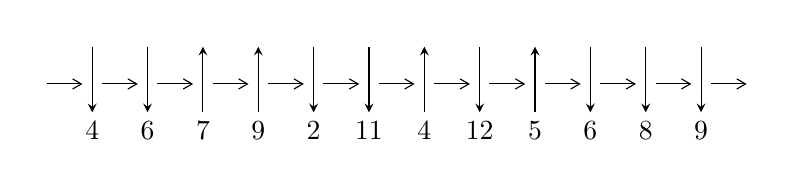
\begin{tikzpicture}[x=20pt, y=17pt]
	% nodes
	\node (C0) at (0, 0) {};
	\node (C1) at (1, 0) {};
	\node (C1U) at (1, +1) {};
	\node (C1D) at (1, -1) {4};

	\node (C2) at (2, 0) {};
	\node (C2U) at (2, +1) {};
	\node (C2D) at (2, -1) {6};

	\node (C3) at (3, 0) {};
	\node (C3U) at (3, +1) {};
	\node (C3D) at (3, -1) {7};

	\node (C4) at (4, 0) {};
	\node (C4U) at (4, +1) {};
	\node (C4D) at (4, -1) {9};

	\node (C5) at (5, 0) {};
	\node (C5U) at (5, +1) {};
	\node (C5D) at (5, -1) {2};

	\node (C6) at (6, 0) {};
	\node (C6U) at (6, +1) {};
	\node (C6D) at (6, -1) {11};

	\node (C7) at (7, 0) {};
	\node (C7U) at (7, +1) {};
	\node (C7D) at (7, -1) {4};

	\node (C8) at (8, 0) {};
	\node (C8U) at (8, +1) {};
	\node (C8D) at (8, -1) {12};

	\node (C9) at (9, 0) {};
	\node (C9U) at (9, +1) {};
	\node (C9D) at (9, -1) {5};

	\node (C10) at (10, 0) {};
	\node (C10U) at (10, +1) {};
	\node (C10D) at (10, -1) {6};

	\node (C11) at (11, 0) {};
	\node (C11U) at (11, +1) {};
	\node (C11D) at (11, -1) {8};

	\node (C12) at (12, 0) {};
	\node (C12U) at (12, +1) {};
	\node (C12D) at (12, -1) {9};
	\node (C13) at (13, 0) {};

	% arrows
	\draw[->,>={angle 60}]
	(C0) edge (C1) (C1) edge (C2) (C2) edge (C3) (C3) edge (C4) (C4) edge (C5) (C5) edge (C6) (C6) edge (C7) (C7) edge (C8) (C8) edge (C9) (C9) edge (C10) (C10) edge (C11) (C11) edge (C12) (C12) edge (C13) ;	\draw[->,>=stealth]
	(C1U) edge (C1D) (C2U) edge (C2D) (C3D) edge (C3U) (C4D) edge (C4U) (C5U) edge (C5D) (C6U) edge (C6D) (C7D) edge (C7U) (C8U) edge (C8D) (C9D) edge (C9U) (C10U) edge (C10D) (C11U) edge (C11D) (C12U) edge (C12D) ;
	\end{tikzpicture} \\
\hhline{~~} \\& 
\textbf{Solving Sequence} \\ \cline{2-2} 
 &
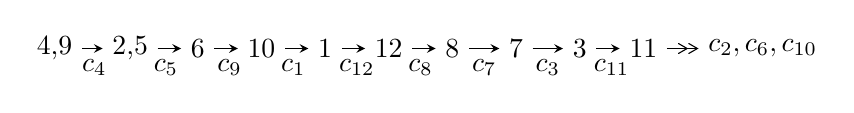
\begin{tikzpicture}[x=23pt, y=7pt]
	% node
	\node (A0) at (-1/8, 0) {4,9};
	\node (A1) at (17/16, 0) {2,5};
	\node (A2) at (17/8, 0) {6};
	\node (A3) at (25/8, 0) {10};
	\node (A4) at (33/8, 0) {1};
	\node (A5) at (41/8, 0) {12};
	\node (A6) at (49/8, 0) {8};
	\node (A7) at (57/8, 0) {7};
	\node (A8) at (65/8, 0) {3};
	\node (A9) at (73/8, 0) {11};
	\node (C1) at (1/2, -1) {$c_{4}$};
	\node (C2) at (13/8, -1) {$c_{5}$};
	\node (C3) at (21/8, -1) {$c_{9}$};
	\node (C4) at (29/8, -1) {$c_{1}$};
	\node (C5) at (37/8, -1) {$c_{12}$};
	\node (C6) at (45/8, -1) {$c_{8}$};
	\node (C7) at (53/8, -1) {$c_{7}$};
	\node (C8) at (61/8, -1) {$c_{3}$};
	\node (C9) at (69/8, -1) {$c_{11}$};
	\node (A10) at (11, 0) {$c_{2},c_{6},c_{10}$};

	% edge
	\draw[->,>=stealth]	
	(A0) edge (A1) (A1) edge (A2) (A2) edge (A3) (A3) edge (A4) (A4) edge (A5) (A5) edge (A6) (A6) edge (A7) (A7) edge (A8) (A8) edge (A9) ;
	\draw[->>,>={angle 60}]	
	(A9) edge (A10);
\end{tikzpicture} \\ 

\end{tabular} \\

\footnotetext{
The image of knot diagram is generated by the software ``\textbf{Draw programme}" developed by Andrew Bartholomew(\url{http://www.layer8.co.uk/maths/draw/index.htm\#Running-draw}), where we modified some parts for our purpose(\url{https://github.com/CATsTAILs/LinksPainter}).
}\phantom \\ \newline 
\centering \textbf{Ideals for irreducible components\footnotemark of $X_{\text{par}}$} 
 
\begin{align*}
I^u_{1}&=\langle 
5.55332\times10^{75} u^{50}+2.14999\times10^{75} u^{49}+\cdots+1.63199\times10^{76} b-9.50449\times10^{76},\\
\phantom{I^u_{1}}&\phantom{= \langle  }-1.00920\times10^{77} u^{50}-6.14195\times10^{76} u^{49}+\cdots+4.89597\times10^{76} a+2.60239\times10^{78},\;u^{51}+u^{50}+\cdots+9 u-9\rangle \\
I^u_{2}&=\langle 
u^{11}+3 u^{10}-6 u^9-5 u^8+19 u^7-14 u^6-34 u^5+34 u^4+25 u^3-24 u^2+5 b+u+8,\\
\phantom{I^u_{2}}&\phantom{= \langle  }-19 u^{11}+3 u^{10}+89 u^9-75 u^8-136 u^7+321 u^6+41 u^5-531 u^4+80 u^3+341 u^2+5 a-64 u-47,\\
\phantom{I^u_{2}}&\phantom{= \langle  }u^{12}-5 u^{10}+3 u^9+9 u^8-16 u^7-7 u^6+31 u^5+3 u^4-24 u^3-2 u^2+5 u+1\rangle \\
\\
\end{align*}
\raggedright * 2 irreducible components of $\dim_{\mathbb{C}}=0$, with total 63 representations.\\
\footnotetext{All coefficients of polynomials are rational numbers. But the coefficients are sometimes approximated in decimal forms when there is not enough margin.}
\newpage
\renewcommand{\arraystretch}{1}
\centering \section*{I. $I^u_{1}= \langle 5.55\times10^{75} u^{50}+2.15\times10^{75} u^{49}+\cdots+1.63\times10^{76} b-9.50\times10^{76},\;-1.01\times10^{77} u^{50}-6.14\times10^{76} u^{49}+\cdots+4.90\times10^{76} a+2.60\times10^{78},\;u^{51}+u^{50}+\cdots+9 u-9 \rangle$}
\flushleft \textbf{(i) Arc colorings}\\
\begin{tabular}{m{7pt} m{180pt} m{7pt} m{180pt} }
\flushright $a_{4}=$&$\begin{pmatrix}1\\0\end{pmatrix}$ \\
\flushright $a_{9}=$&$\begin{pmatrix}0\\u\end{pmatrix}$ \\
\flushright $a_{2}=$&$\begin{pmatrix}2.06129 u^{50}+1.25449 u^{49}+\cdots+156.424 u-53.1538\\-0.340279 u^{50}-0.131740 u^{49}+\cdots-5.95216 u+5.82387\end{pmatrix}$ \\
\flushright $a_{5}=$&$\begin{pmatrix}1\\- u^2\end{pmatrix}$ \\
\flushright $a_{6}=$&$\begin{pmatrix}-3.63256 u^{50}-2.37017 u^{49}+\cdots-340.652 u+80.1409\\-0.228512 u^{50}-0.176770 u^{49}+\cdots-38.9007 u+9.50612\end{pmatrix}$ \\
\flushright $a_{10}=$&$\begin{pmatrix}u\\- u^3+u\end{pmatrix}$ \\
\flushright $a_{1}=$&$\begin{pmatrix}1.72101 u^{50}+1.12275 u^{49}+\cdots+150.472 u-47.3299\\-0.340279 u^{50}-0.131740 u^{49}+\cdots-5.95216 u+5.82387\end{pmatrix}$ \\
\flushright $a_{12}=$&$\begin{pmatrix}1.72101 u^{50}+1.12275 u^{49}+\cdots+150.472 u-47.3299\\-0.570525 u^{50}-0.285333 u^{49}+\cdots-26.8255 u+11.2082\end{pmatrix}$ \\
\flushright $a_{8}=$&$\begin{pmatrix}3.13695 u^{50}+1.91795 u^{49}+\cdots+298.052 u-76.5104\\0.639941 u^{50}+0.374469 u^{49}+\cdots+59.0371 u-16.4493\end{pmatrix}$ \\
\flushright $a_{7}=$&$\begin{pmatrix}2.49701 u^{50}+1.54348 u^{49}+\cdots+239.015 u-60.0611\\0.639941 u^{50}+0.374469 u^{49}+\cdots+59.0371 u-16.4493\end{pmatrix}$ \\
\flushright $a_{3}=$&$\begin{pmatrix}-3.39441 u^{50}-1.99256 u^{49}+\cdots-330.150 u+85.1843\\-1.49048 u^{50}-1.03131 u^{49}+\cdots-138.506 u+38.2645\end{pmatrix}$ \\
\flushright $a_{11}=$&$\begin{pmatrix}-2.02479 u^{50}-1.32882 u^{49}+\cdots-189.222 u+38.3733\\-1.71640 u^{50}-1.07355 u^{49}+\cdots-148.388 u+42.1932\end{pmatrix}$\\&\end{tabular}
\flushleft \textbf{(ii) Obstruction class $= -1$}\\~\\
\flushleft \textbf{(iii) Cusp Shapes $= 23.5676 u^{50}+14.4075 u^{49}+\cdots+1956.28 u-544.212$}\\~\\
\newpage\renewcommand{\arraystretch}{1}
\flushleft \textbf{(iv) u-Polynomials at the component}\newline \\
\begin{tabular}{m{50pt}|m{274pt}}
Crossings & \hspace{64pt}u-Polynomials at each crossing \\
\hline $$\begin{aligned}c_{1}\end{aligned}$$&$\begin{aligned}
&u^{51}-2 u^{50}+\cdots-2798 u-211
\end{aligned}$\\
\hline $$\begin{aligned}c_{2},c_{5}\end{aligned}$$&$\begin{aligned}
&u^{51}+2 u^{50}+\cdots-10 u+1
\end{aligned}$\\
\hline $$\begin{aligned}c_{3},c_{7}\end{aligned}$$&$\begin{aligned}
&u^{51}-2 u^{50}+\cdots-110 u-11
\end{aligned}$\\
\hline $$\begin{aligned}c_{4},c_{9}\end{aligned}$$&$\begin{aligned}
&u^{51}+u^{50}+\cdots+9 u-9
\end{aligned}$\\
\hline $$\begin{aligned}c_{6},c_{10}\end{aligned}$$&$\begin{aligned}
&u^{51}-2 u^{50}+\cdots-17 u+1
\end{aligned}$\\
\hline $$\begin{aligned}c_{8},c_{11},c_{12}\end{aligned}$$&$\begin{aligned}
&u^{51}-18 u^{49}+\cdots+13 u-1
\end{aligned}$\\
\hline
\end{tabular}\\~\\
\newpage\renewcommand{\arraystretch}{1}
\flushleft \textbf{(v) Riley Polynomials at the component}\newline \\
\begin{tabular}{m{50pt}|m{274pt}}
Crossings & \hspace{64pt}Riley Polynomials at each crossing \\
\hline $$\begin{aligned}c_{1}\end{aligned}$$&$\begin{aligned}
&y^{51}+70 y^{50}+\cdots+9533684 y-44521
\end{aligned}$\\
\hline $$\begin{aligned}c_{2},c_{5}\end{aligned}$$&$\begin{aligned}
&y^{51}-10 y^{50}+\cdots+26 y-1
\end{aligned}$\\
\hline $$\begin{aligned}c_{3},c_{7}\end{aligned}$$&$\begin{aligned}
&y^{51}-40 y^{50}+\cdots+12914 y-121
\end{aligned}$\\
\hline $$\begin{aligned}c_{4},c_{9}\end{aligned}$$&$\begin{aligned}
&y^{51}-51 y^{50}+\cdots+6489 y-81
\end{aligned}$\\
\hline $$\begin{aligned}c_{6},c_{10}\end{aligned}$$&$\begin{aligned}
&y^{51}-8 y^{50}+\cdots+181 y-1
\end{aligned}$\\
\hline $$\begin{aligned}c_{8},c_{11},c_{12}\end{aligned}$$&$\begin{aligned}
&y^{51}-36 y^{50}+\cdots+279 y-1
\end{aligned}$\\
\hline
\end{tabular}\\~\\
\newpage\flushleft \textbf{(vi) Complex Volumes and Cusp Shapes}
$$\begin{array}{c|c|c}  
\text{Solutions to }I^u_{1}& \I (\text{vol} + \sqrt{-1}CS) & \text{Cusp shape}\\
 \hline 
\begin{aligned}
u &= \phantom{-}0.966312 + 0.028011 I \\
a &= -0.536822 - 0.279028 I \\
b &= \phantom{-}0.882354 - 0.296412 I\end{aligned}
 & \phantom{-}3.13672 - 0.62690 I & \phantom{-0.000000 } 0 \\ \hline\begin{aligned}
u &= \phantom{-}0.966312 - 0.028011 I \\
a &= -0.536822 + 0.279028 I \\
b &= \phantom{-}0.882354 + 0.296412 I\end{aligned}
 & \phantom{-}3.13672 + 0.62690 I & \phantom{-0.000000 } 0 \\ \hline\begin{aligned}
u &= -0.752807 + 0.539036 I \\
a &= -0.872796 + 0.719742 I \\
b &= \phantom{-}0.459364 - 0.125960 I\end{aligned}
 & \phantom{-}2.93432 - 5.19831 I & \phantom{-0.000000 -}0. + 6.04454 I \\ \hline\begin{aligned}
u &= -0.752807 - 0.539036 I \\
a &= -0.872796 - 0.719742 I \\
b &= \phantom{-}0.459364 + 0.125960 I\end{aligned}
 & \phantom{-}2.93432 + 5.19831 I & \phantom{-0.000000 } 0. - 6.04454 I \\ \hline\begin{aligned}
u &= \phantom{-}1.08285\phantom{ +0.000000I} \\
a &= -0.166192\phantom{ +0.000000I} \\
b &= -1.36678\phantom{ +0.000000I}\end{aligned}
 & -8.81786\phantom{ +0.000000I} & \phantom{-0.000000 } 0 \\ \hline\begin{aligned}
u &= -0.237795 + 0.803808 I \\
a &= \phantom{-}0.997700 + 0.304588 I \\
b &= -0.237661 + 0.548165 I\end{aligned}
 & -1.59127 + 1.64954 I & -10.79264 - 4.97589 I \\ \hline\begin{aligned}
u &= -0.237795 - 0.803808 I \\
a &= \phantom{-}0.997700 - 0.304588 I \\
b &= -0.237661 - 0.548165 I\end{aligned}
 & -1.59127 - 1.64954 I & -10.79264 + 4.97589 I \\ \hline\begin{aligned}
u &= -1.229440 + 0.096772 I \\
a &= -0.45337 + 1.83496 I \\
b &= \phantom{-}0.96203 - 1.87253 I\end{aligned}
 & \phantom{-}3.25985 - 4.40630 I & \phantom{-0.000000 } 0 \\ \hline\begin{aligned}
u &= -1.229440 - 0.096772 I \\
a &= -0.45337 - 1.83496 I \\
b &= \phantom{-}0.96203 + 1.87253 I\end{aligned}
 & \phantom{-}3.25985 + 4.40630 I & \phantom{-0.000000 } 0 \\ \hline\begin{aligned}
u &= -1.23712\phantom{ +0.000000I} \\
a &= \phantom{-}1.45818\phantom{ +0.000000I} \\
b &= -0.238614\phantom{ +0.000000I}\end{aligned}
 & -3.66174\phantom{ +0.000000I} & \phantom{-0.000000 } 0\\
 \hline 
 \end{array}$$\newpage$$\begin{array}{c|c|c}  
\text{Solutions to }I^u_{1}& \I (\text{vol} + \sqrt{-1}CS) & \text{Cusp shape}\\
 \hline 
\begin{aligned}
u &= -0.205562 + 0.732617 I \\
a &= \phantom{-}0.314612 - 0.527449 I \\
b &= -0.548118 - 0.948146 I\end{aligned}
 & -3.85278 - 3.00372 I & -11.66965 + 6.00585 I \\ \hline\begin{aligned}
u &= -0.205562 - 0.732617 I \\
a &= \phantom{-}0.314612 + 0.527449 I \\
b &= -0.548118 + 0.948146 I\end{aligned}
 & -3.85278 + 3.00372 I & -11.66965 - 6.00585 I \\ \hline\begin{aligned}
u &= \phantom{-}0.572928 + 1.104770 I \\
a &= -0.206310 - 0.298977 I \\
b &= \phantom{-}0.320739 - 0.725671 I\end{aligned}
 & -0.44013 + 9.46101 I & \phantom{-0.000000 } 0 \\ \hline\begin{aligned}
u &= \phantom{-}0.572928 - 1.104770 I \\
a &= -0.206310 + 0.298977 I \\
b &= \phantom{-}0.320739 + 0.725671 I\end{aligned}
 & -0.44013 - 9.46101 I & \phantom{-0.000000 } 0 \\ \hline\begin{aligned}
u &= -1.223810 + 0.312977 I \\
a &= -0.32338 + 1.52316 I \\
b &= -0.38353 - 2.16692 I\end{aligned}
 & \phantom{-}1.53528 - 5.83376 I & \phantom{-0.000000 } 0 \\ \hline\begin{aligned}
u &= -1.223810 - 0.312977 I \\
a &= -0.32338 - 1.52316 I \\
b &= -0.38353 + 2.16692 I\end{aligned}
 & \phantom{-}1.53528 + 5.83376 I & \phantom{-0.000000 } 0 \\ \hline\begin{aligned}
u &= \phantom{-}1.304010 + 0.126559 I \\
a &= -0.351078 - 0.800505 I \\
b &= \phantom{-}0.73472 + 1.28447 I\end{aligned}
 & \phantom{-}3.37052 + 0.99994 I & \phantom{-0.000000 } 0 \\ \hline\begin{aligned}
u &= \phantom{-}1.304010 - 0.126559 I \\
a &= -0.351078 + 0.800505 I \\
b &= \phantom{-}0.73472 - 1.28447 I\end{aligned}
 & \phantom{-}3.37052 - 0.99994 I & \phantom{-0.000000 } 0 \\ \hline\begin{aligned}
u &= -1.289750 + 0.452317 I \\
a &= \phantom{-}0.550918 - 0.357255 I \\
b &= \phantom{-}0.193129 + 0.814567 I\end{aligned}
 & -1.04630 - 1.13129 I & \phantom{-0.000000 } 0 \\ \hline\begin{aligned}
u &= -1.289750 - 0.452317 I \\
a &= \phantom{-}0.550918 + 0.357255 I \\
b &= \phantom{-}0.193129 - 0.814567 I\end{aligned}
 & -1.04630 + 1.13129 I & \phantom{-0.000000 } 0\\
 \hline 
 \end{array}$$\newpage$$\begin{array}{c|c|c}  
\text{Solutions to }I^u_{1}& \I (\text{vol} + \sqrt{-1}CS) & \text{Cusp shape}\\
 \hline 
\begin{aligned}
u &= \phantom{-}0.131606 + 0.597948 I \\
a &= \phantom{-}0.755619 + 0.012297 I \\
b &= -0.236259 + 0.347071 I\end{aligned}
 & -0.317906 + 1.195420 I & -3.90544 - 5.43225 I \\ \hline\begin{aligned}
u &= \phantom{-}0.131606 - 0.597948 I \\
a &= \phantom{-}0.755619 - 0.012297 I \\
b &= -0.236259 - 0.347071 I\end{aligned}
 & -0.317906 - 1.195420 I & -3.90544 + 5.43225 I \\ \hline\begin{aligned}
u &= \phantom{-}1.385030 + 0.283021 I \\
a &= \phantom{-}0.04231 - 1.92490 I \\
b &= -0.77123 + 2.30254 I\end{aligned}
 & \phantom{-}1.21275 + 6.65866 I & \phantom{-0.000000 } 0 \\ \hline\begin{aligned}
u &= \phantom{-}1.385030 - 0.283021 I \\
a &= \phantom{-}0.04231 + 1.92490 I \\
b &= -0.77123 - 2.30254 I\end{aligned}
 & \phantom{-}1.21275 - 6.65866 I & \phantom{-0.000000 } 0 \\ \hline\begin{aligned}
u &= -1.46412 + 0.01784 I \\
a &= -0.244361 - 1.204180 I \\
b &= -0.79728 + 1.66527 I\end{aligned}
 & \phantom{-}5.76286 - 1.13846 I & \phantom{-0.000000 } 0 \\ \hline\begin{aligned}
u &= -1.46412 - 0.01784 I \\
a &= -0.244361 + 1.204180 I \\
b &= -0.79728 - 1.66527 I\end{aligned}
 & \phantom{-}5.76286 + 1.13846 I & \phantom{-0.000000 } 0 \\ \hline\begin{aligned}
u &= \phantom{-}0.514876\phantom{ +0.000000I} \\
a &= \phantom{-}3.02685\phantom{ +0.000000I} \\
b &= \phantom{-}0.317888\phantom{ +0.000000I}\end{aligned}
 & -10.7307\phantom{ +0.000000I} & \phantom{-}10.2750\phantom{ +0.000000I} \\ \hline\begin{aligned}
u &= \phantom{-}1.48372 + 0.08688 I \\
a &= \phantom{-}0.167132 - 1.009410 I \\
b &= \phantom{-}0.37784 + 1.38305 I\end{aligned}
 & \phantom{-}4.37936 + 0.98278 I & \phantom{-0.000000 } 0 \\ \hline\begin{aligned}
u &= \phantom{-}1.48372 - 0.08688 I \\
a &= \phantom{-}0.167132 + 1.009410 I \\
b &= \phantom{-}0.37784 - 1.38305 I\end{aligned}
 & \phantom{-}4.37936 - 0.98278 I & \phantom{-0.000000 } 0 \\ \hline\begin{aligned}
u &= \phantom{-}1.49336 + 0.11013 I \\
a &= -0.41151 - 1.40552 I \\
b &= -0.51248 + 1.86936 I\end{aligned}
 & \phantom{-}7.35814 + 6.04698 I & \phantom{-0.000000 } 0\\
 \hline 
 \end{array}$$\newpage$$\begin{array}{c|c|c}  
\text{Solutions to }I^u_{1}& \I (\text{vol} + \sqrt{-1}CS) & \text{Cusp shape}\\
 \hline 
\begin{aligned}
u &= \phantom{-}1.49336 - 0.11013 I \\
a &= -0.41151 + 1.40552 I \\
b &= -0.51248 - 1.86936 I\end{aligned}
 & \phantom{-}7.35814 - 6.04698 I & \phantom{-0.000000 } 0 \\ \hline\begin{aligned}
u &= -0.491947\phantom{ +0.000000I} \\
a &= \phantom{-}1.66651\phantom{ +0.000000I} \\
b &= -0.0705730\phantom{ +0.000000I}\end{aligned}
 & -1.36137\phantom{ +0.000000I} & -6.25410\phantom{ +0.000000I} \\ \hline\begin{aligned}
u &= -0.399561 + 0.244629 I \\
a &= -2.11272 - 0.74059 I \\
b &= \phantom{-}0.615884 - 1.246730 I\end{aligned}
 & \phantom{-}1.00696 - 4.56920 I & -3.90257 + 5.25320 I \\ \hline\begin{aligned}
u &= -0.399561 - 0.244629 I \\
a &= -2.11272 + 0.74059 I \\
b &= \phantom{-}0.615884 + 1.246730 I\end{aligned}
 & \phantom{-}1.00696 + 4.56920 I & -3.90257 - 5.25320 I \\ \hline\begin{aligned}
u &= -1.50785 + 0.38384 I \\
a &= -0.017099 + 1.147920 I \\
b &= -0.35140 - 1.57334 I\end{aligned}
 & \phantom{-}4.58888 - 5.41893 I & \phantom{-0.000000 } 0 \\ \hline\begin{aligned}
u &= -1.50785 - 0.38384 I \\
a &= -0.017099 - 1.147920 I \\
b &= -0.35140 + 1.57334 I\end{aligned}
 & \phantom{-}4.58888 + 5.41893 I & \phantom{-0.000000 } 0 \\ \hline\begin{aligned}
u &= \phantom{-}1.57518 + 0.19913 I \\
a &= -0.200647 + 1.350350 I \\
b &= \phantom{-}0.06483 - 2.13765 I\end{aligned}
 & \phantom{-}10.54910 + 8.09027 I & \phantom{-0.000000 } 0 \\ \hline\begin{aligned}
u &= \phantom{-}1.57518 - 0.19913 I \\
a &= -0.200647 - 1.350350 I \\
b &= \phantom{-}0.06483 + 2.13765 I\end{aligned}
 & \phantom{-}10.54910 - 8.09027 I & \phantom{-0.000000 } 0 \\ \hline\begin{aligned}
u &= -0.407564\phantom{ +0.000000I} \\
a &= \phantom{-}1.19912\phantom{ +0.000000I} \\
b &= -1.34717\phantom{ +0.000000I}\end{aligned}
 & -2.57791\phantom{ +0.000000I} & \phantom{-}9.00240\phantom{ +0.000000I} \\ \hline\begin{aligned}
u &= -1.61819 + 0.08048 I \\
a &= -0.265175 - 1.291110 I \\
b &= \phantom{-}0.19764 + 2.01735 I\end{aligned}
 & \phantom{-}11.95830 - 0.22760 I & \phantom{-0.000000 } 0\\
 \hline 
 \end{array}$$\newpage$$\begin{array}{c|c|c}  
\text{Solutions to }I^u_{1}& \I (\text{vol} + \sqrt{-1}CS) & \text{Cusp shape}\\
 \hline 
\begin{aligned}
u &= -1.61819 - 0.08048 I \\
a &= -0.265175 + 1.291110 I \\
b &= \phantom{-}0.19764 - 2.01735 I\end{aligned}
 & \phantom{-}11.95830 + 0.22760 I & \phantom{-0.000000 } 0 \\ \hline\begin{aligned}
u &= -1.58168 + 0.38198 I \\
a &= -0.17902 - 1.40951 I \\
b &= \phantom{-}0.91256 + 2.00149 I\end{aligned}
 & \phantom{-}6.4507 - 14.7902 I & \phantom{-0.000000 } 0 \\ \hline\begin{aligned}
u &= -1.58168 - 0.38198 I \\
a &= -0.17902 + 1.40951 I \\
b &= \phantom{-}0.91256 - 2.00149 I\end{aligned}
 & \phantom{-}6.4507 + 14.7902 I & \phantom{-0.000000 } 0 \\ \hline\begin{aligned}
u &= -0.364492\phantom{ +0.000000I} \\
a &= -2.15420\phantom{ +0.000000I} \\
b &= -1.45022\phantom{ +0.000000I}\end{aligned}
 & -6.63015\phantom{ +0.000000I} & -21.7480\phantom{ +0.000000I} \\ \hline\begin{aligned}
u &= \phantom{-}1.63613 + 0.31897 I \\
a &= -0.126349 + 1.180690 I \\
b &= \phantom{-}0.85837 - 1.71259 I\end{aligned}
 & \phantom{-}7.91149 + 6.61409 I & \phantom{-0.000000 } 0 \\ \hline\begin{aligned}
u &= \phantom{-}1.63613 - 0.31897 I \\
a &= -0.126349 - 1.180690 I \\
b &= \phantom{-}0.85837 + 1.71259 I\end{aligned}
 & \phantom{-}7.91149 - 6.61409 I & \phantom{-0.000000 } 0 \\ \hline\begin{aligned}
u &= \phantom{-}0.169849 + 0.057002 I \\
a &= -7.63550 - 0.35036 I \\
b &= \phantom{-}0.860446 - 0.474071 I\end{aligned}
 & \phantom{-}0.100763 + 0.877365 I & -4.31516 - 3.77329 I \\ \hline\begin{aligned}
u &= \phantom{-}0.169849 - 0.057002 I \\
a &= -7.63550 + 0.35036 I \\
b &= \phantom{-}0.860446 + 0.474071 I\end{aligned}
 & \phantom{-}0.100763 - 0.877365 I & -4.31516 + 3.77329 I \\ \hline\begin{aligned}
u &= \phantom{-}1.87867\phantom{ +0.000000I} \\
a &= \phantom{-}0.431311\phantom{ +0.000000I} \\
b &= -0.853122\phantom{ +0.000000I}\end{aligned}
 & \phantom{-}1.07210\phantom{ +0.000000I} & \phantom{-0.000000 } 0 \\ \hline\begin{aligned}
u &= -0.19520 + 1.90391 I \\
a &= \phantom{-}0.0437236 + 0.0504691 I \\
b &= -0.097631 + 0.463019 I\end{aligned}
 & -0.098440 - 0.706098 I & \phantom{-0.000000 } 0\\
 \hline 
 \end{array}$$\newpage$$\begin{array}{c|c|c}  
\text{Solutions to }I^u_{1}& \I (\text{vol} + \sqrt{-1}CS) & \text{Cusp shape}\\
 \hline 
\begin{aligned}
u &= -0.19520 - 1.90391 I \\
a &= \phantom{-}0.0437236 - 0.0504691 I \\
b &= -0.097631 - 0.463019 I\end{aligned}
 & -0.098440 + 0.706098 I & \phantom{-0.000000 } 0\\
 \hline 
 \end{array}$$\newpage\newpage\renewcommand{\arraystretch}{1}
\centering \section*{II. $I^u_{2}= \langle u^{11}+3 u^{10}+\cdots+5 b+8,\;-19 u^{11}+3 u^{10}+\cdots+5 a-47,\;u^{12}-5 u^{10}+\cdots+5 u+1 \rangle$}
\flushleft \textbf{(i) Arc colorings}\\
\begin{tabular}{m{7pt} m{180pt} m{7pt} m{180pt} }
\flushright $a_{4}=$&$\begin{pmatrix}1\\0\end{pmatrix}$ \\
\flushright $a_{9}=$&$\begin{pmatrix}0\\u\end{pmatrix}$ \\
\flushright $a_{2}=$&$\begin{pmatrix}\frac{19}{5} u^{11}-\frac{3}{5} u^{10}+\cdots+\frac{64}{5} u+\frac{47}{5}\\-\frac{1}{5} u^{11}-\frac{3}{5} u^{10}+\cdots-\frac{1}{5} u-\frac{8}{5}\end{pmatrix}$ \\
\flushright $a_{5}=$&$\begin{pmatrix}1\\- u^2\end{pmatrix}$ \\
\flushright $a_{6}=$&$\begin{pmatrix}-\frac{12}{5} u^{11}+\frac{9}{5} u^{10}+\cdots-\frac{97}{5} u-\frac{51}{5}\\-\frac{2}{5} u^{11}-\frac{6}{5} u^{10}+\cdots+\frac{33}{5} u+\frac{14}{5}\end{pmatrix}$ \\
\flushright $a_{10}=$&$\begin{pmatrix}u\\- u^3+u\end{pmatrix}$ \\
\flushright $a_{1}=$&$\begin{pmatrix}\frac{18}{5} u^{11}-\frac{6}{5} u^{10}+\cdots+\frac{63}{5} u+\frac{39}{5}\\-\frac{1}{5} u^{11}-\frac{3}{5} u^{10}+\cdots-\frac{1}{5} u-\frac{8}{5}\end{pmatrix}$ \\
\flushright $a_{12}=$&$\begin{pmatrix}\frac{18}{5} u^{11}-\frac{6}{5} u^{10}+\cdots+\frac{63}{5} u+\frac{39}{5}\\-\frac{8}{5} u^{11}+\frac{1}{5} u^{10}+\cdots-\frac{13}{5} u-\frac{14}{5}\end{pmatrix}$ \\
\flushright $a_{8}=$&$\begin{pmatrix}\frac{11}{5} u^{11}-\frac{2}{5} u^{10}+\cdots+\frac{101}{5} u+\frac{33}{5}\\-\frac{2}{5} u^{11}-\frac{6}{5} u^{10}+\cdots+\frac{33}{5} u+\frac{9}{5}\end{pmatrix}$ \\
\flushright $a_{7}=$&$\begin{pmatrix}\frac{13}{5} u^{11}+\frac{4}{5} u^{10}+\cdots+\frac{68}{5} u+\frac{24}{5}\\-\frac{2}{5} u^{11}-\frac{6}{5} u^{10}+\cdots+\frac{33}{5} u+\frac{9}{5}\end{pmatrix}$ \\
\flushright $a_{3}=$&$\begin{pmatrix}-\frac{17}{5} u^{11}-\frac{6}{5} u^{10}+\cdots+\frac{18}{5} u-\frac{1}{5}\\\frac{3}{5} u^{11}+\frac{4}{5} u^{10}+\cdots-\frac{7}{5} u-\frac{1}{5}\end{pmatrix}$ \\
\flushright $a_{11}=$&$\begin{pmatrix}-\frac{22}{5} u^{11}+\frac{9}{5} u^{10}+\cdots-\frac{97}{5} u-\frac{31}{5}\\-\frac{3}{5} u^{11}+\frac{1}{5} u^{10}+\cdots-\frac{13}{5} u-\frac{14}{5}\end{pmatrix}$\\&\end{tabular}
\flushleft \textbf{(ii) Obstruction class $= 1$}\\~\\
\flushleft \textbf{(iii) Cusp Shapes $= -\frac{1}{5} u^{11}-\frac{33}{5} u^{10}-\frac{9}{5} u^9+27 u^8-\frac{74}{5} u^7-\frac{216}{5} u^6+\frac{439}{5} u^5+\frac{176}{5} u^4-135 u^3-\frac{71}{5} u^2+\frac{294}{5} u-\frac{43}{5}$}\\~\\
\newpage\renewcommand{\arraystretch}{1}
\flushleft \textbf{(iv) u-Polynomials at the component}\newline \\
\begin{tabular}{m{50pt}|m{274pt}}
Crossings & \hspace{64pt}u-Polynomials at each crossing \\
\hline $$\begin{aligned}c_{1}\end{aligned}$$&$\begin{aligned}
&u^{12}- u^{11}+\cdots+6 u-1
\end{aligned}$\\
\hline $$\begin{aligned}c_{2}\end{aligned}$$&$\begin{aligned}
&u^{12}+3 u^{11}+\cdots+2 u-1
\end{aligned}$\\
\hline $$\begin{aligned}c_{3}\end{aligned}$$&$\begin{aligned}
&u^{12}- u^{11}+\cdots+15 u^2-1
\end{aligned}$\\
\hline $$\begin{aligned}c_{4}\end{aligned}$$&$\begin{aligned}
&u^{12}-5 u^{10}+\cdots+5 u+1
\end{aligned}$\\
\hline $$\begin{aligned}c_{5}\end{aligned}$$&$\begin{aligned}
&u^{12}-3 u^{11}+\cdots-2 u-1
\end{aligned}$\\
\hline $$\begin{aligned}c_{6}\end{aligned}$$&$\begin{aligned}
&u^{12}- u^{11}+\cdots+u-1
\end{aligned}$\\
\hline $$\begin{aligned}c_{7}\end{aligned}$$&$\begin{aligned}
&u^{12}+u^{11}+\cdots+15 u^2-1
\end{aligned}$\\
\hline $$\begin{aligned}c_{8}\end{aligned}$$&$\begin{aligned}
&u^{12}+u^{11}+\cdots-5 u+1
\end{aligned}$\\
\hline $$\begin{aligned}c_{9}\end{aligned}$$&$\begin{aligned}
&u^{12}-5 u^{10}+\cdots-5 u+1
\end{aligned}$\\
\hline $$\begin{aligned}c_{10}\end{aligned}$$&$\begin{aligned}
&u^{12}+u^{11}+\cdots- u-1
\end{aligned}$\\
\hline $$\begin{aligned}c_{11},c_{12}\end{aligned}$$&$\begin{aligned}
&u^{12}- u^{11}+\cdots+5 u+1
\end{aligned}$\\
\hline
\end{tabular}\\~\\
\newpage\renewcommand{\arraystretch}{1}
\flushleft \textbf{(v) Riley Polynomials at the component}\newline \\
\begin{tabular}{m{50pt}|m{274pt}}
Crossings & \hspace{64pt}Riley Polynomials at each crossing \\
\hline $$\begin{aligned}c_{1}\end{aligned}$$&$\begin{aligned}
&y^{12}+7 y^{11}+\cdots-4 y+1
\end{aligned}$\\
\hline $$\begin{aligned}c_{2},c_{5}\end{aligned}$$&$\begin{aligned}
&y^{12}-13 y^{11}+\cdots-6 y+1
\end{aligned}$\\
\hline $$\begin{aligned}c_{3},c_{7}\end{aligned}$$&$\begin{aligned}
&y^{12}-11 y^{11}+\cdots-30 y+1
\end{aligned}$\\
\hline $$\begin{aligned}c_{4},c_{9}\end{aligned}$$&$\begin{aligned}
&y^{12}-10 y^{11}+\cdots-29 y+1
\end{aligned}$\\
\hline $$\begin{aligned}c_{6},c_{10}\end{aligned}$$&$\begin{aligned}
&y^{12}-7 y^{11}+\cdots-13 y+1
\end{aligned}$\\
\hline $$\begin{aligned}c_{8},c_{11},c_{12}\end{aligned}$$&$\begin{aligned}
&y^{12}-15 y^{11}+\cdots-27 y+1
\end{aligned}$\\
\hline
\end{tabular}\\~\\
\newpage\flushleft \textbf{(vi) Complex Volumes and Cusp Shapes}
$$\begin{array}{c|c|c}  
\text{Solutions to }I^u_{2}& \I (\text{vol} + \sqrt{-1}CS) & \text{Cusp shape}\\
 \hline 
\begin{aligned}
u &= \phantom{-}1.21822\phantom{ +0.000000I} \\
a &= \phantom{-}1.79757\phantom{ +0.000000I} \\
b &= -0.601851\phantom{ +0.000000I}\end{aligned}
 & -4.03710\phantom{ +0.000000I} & -18.0780\phantom{ +0.000000I} \\ \hline\begin{aligned}
u &= -1.27309\phantom{ +0.000000I} \\
a &= \phantom{-}0.277397\phantom{ +0.000000I} \\
b &= \phantom{-}1.16135\phantom{ +0.000000I}\end{aligned}
 & -7.88309\phantom{ +0.000000I} & -1.62320\phantom{ +0.000000I} \\ \hline\begin{aligned}
u &= -1.268290 + 0.330427 I \\
a &= -0.58188 + 1.78206 I \\
b &= -0.09657 - 2.27913 I\end{aligned}
 & \phantom{-}2.50992 - 6.48574 I & -1.33595 + 8.54705 I \\ \hline\begin{aligned}
u &= -1.268290 - 0.330427 I \\
a &= -0.58188 - 1.78206 I \\
b &= -0.09657 + 2.27913 I\end{aligned}
 & \phantom{-}2.50992 + 6.48574 I & -1.33595 - 8.54705 I \\ \hline\begin{aligned}
u &= \phantom{-}1.320490 + 0.182645 I \\
a &= -0.416916 - 1.142720 I \\
b &= \phantom{-}1.12535 + 1.50126 I\end{aligned}
 & \phantom{-}3.03542 + 2.75700 I & -4.31533 - 2.69611 I \\ \hline\begin{aligned}
u &= \phantom{-}1.320490 - 0.182645 I \\
a &= -0.416916 + 1.142720 I \\
b &= \phantom{-}1.12535 - 1.50126 I\end{aligned}
 & \phantom{-}3.03542 - 2.75700 I & -4.31533 + 2.69611 I \\ \hline\begin{aligned}
u &= \phantom{-}0.638711\phantom{ +0.000000I} \\
a &= -0.671197\phantom{ +0.000000I} \\
b &= -1.41524\phantom{ +0.000000I}\end{aligned}
 & -6.24905\phantom{ +0.000000I} & \phantom{-}0.243470\phantom{ +0.000000I} \\ \hline\begin{aligned}
u &= -1.48898\phantom{ +0.000000I} \\
a &= \phantom{-}0.537683\phantom{ +0.000000I} \\
b &= -0.370407\phantom{ +0.000000I}\end{aligned}
 & \phantom{-}1.74863\phantom{ +0.000000I} & -2.66980\phantom{ +0.000000I} \\ \hline\begin{aligned}
u &= \phantom{-}0.72640 + 1.30991 I \\
a &= -0.191140 + 0.258916 I \\
b &= \phantom{-}0.005412 + 0.445100 I\end{aligned}
 & -0.304228 + 0.769223 I & -12.9708 + 6.3200 I \\ \hline\begin{aligned}
u &= \phantom{-}0.72640 - 1.30991 I \\
a &= -0.191140 - 0.258916 I \\
b &= \phantom{-}0.005412 - 0.445100 I\end{aligned}
 & -0.304228 - 0.769223 I & -12.9708 - 6.3200 I\\
 \hline 
 \end{array}$$\newpage$$\begin{array}{c|c|c}  
\text{Solutions to }I^u_{2}& \I (\text{vol} + \sqrt{-1}CS) & \text{Cusp shape}\\
 \hline 
\begin{aligned}
u &= -0.411452\phantom{ +0.000000I} \\
a &= -3.50522\phantom{ +0.000000I} \\
b &= -0.610386\phantom{ +0.000000I}\end{aligned}
 & -10.9545\phantom{ +0.000000I} & -25.9780\phantom{ +0.000000I} \\ \hline\begin{aligned}
u &= -0.240615\phantom{ +0.000000I} \\
a &= \phantom{-}2.94363\phantom{ +0.000000I} \\
b &= -1.23188\phantom{ +0.000000I}\end{aligned}
 & -2.84629\phantom{ +0.000000I} & -21.6500\phantom{ +0.000000I}\\
 \hline 
 \end{array}$$\newpage
\newpage\renewcommand{\arraystretch}{1}
\centering \section*{ III. u-Polynomials}
\begin{tabular}{m{50pt}|m{274pt}}
Crossings & \hspace{64pt}u-Polynomials at each crossing \\
\hline $$\begin{aligned}c_{1}\end{aligned}$$&$\begin{aligned}
&(u^{12}- u^{11}+\cdots+6 u-1)(u^{51}-2 u^{50}+\cdots-2798 u-211)
\end{aligned}$\\
\hline $$\begin{aligned}c_{2}\end{aligned}$$&$\begin{aligned}
&(u^{12}+3 u^{11}+\cdots+2 u-1)(u^{51}+2 u^{50}+\cdots-10 u+1)
\end{aligned}$\\
\hline $$\begin{aligned}c_{3}\end{aligned}$$&$\begin{aligned}
&(u^{12}- u^{11}+\cdots+15 u^2-1)(u^{51}-2 u^{50}+\cdots-110 u-11)
\end{aligned}$\\
\hline $$\begin{aligned}c_{4}\end{aligned}$$&$\begin{aligned}
&(u^{12}-5 u^{10}+\cdots+5 u+1)(u^{51}+u^{50}+\cdots+9 u-9)
\end{aligned}$\\
\hline $$\begin{aligned}c_{5}\end{aligned}$$&$\begin{aligned}
&(u^{12}-3 u^{11}+\cdots-2 u-1)(u^{51}+2 u^{50}+\cdots-10 u+1)
\end{aligned}$\\
\hline $$\begin{aligned}c_{6}\end{aligned}$$&$\begin{aligned}
&(u^{12}- u^{11}+\cdots+u-1)(u^{51}-2 u^{50}+\cdots-17 u+1)
\end{aligned}$\\
\hline $$\begin{aligned}c_{7}\end{aligned}$$&$\begin{aligned}
&(u^{12}+u^{11}+\cdots+15 u^2-1)(u^{51}-2 u^{50}+\cdots-110 u-11)
\end{aligned}$\\
\hline $$\begin{aligned}c_{8}\end{aligned}$$&$\begin{aligned}
&(u^{12}+u^{11}+\cdots-5 u+1)(u^{51}-18 u^{49}+\cdots+13 u-1)
\end{aligned}$\\
\hline $$\begin{aligned}c_{9}\end{aligned}$$&$\begin{aligned}
&(u^{12}-5 u^{10}+\cdots-5 u+1)(u^{51}+u^{50}+\cdots+9 u-9)
\end{aligned}$\\
\hline $$\begin{aligned}c_{10}\end{aligned}$$&$\begin{aligned}
&(u^{12}+u^{11}+\cdots- u-1)(u^{51}-2 u^{50}+\cdots-17 u+1)
\end{aligned}$\\
\hline $$\begin{aligned}c_{11},c_{12}\end{aligned}$$&$\begin{aligned}
&(u^{12}- u^{11}+\cdots+5 u+1)(u^{51}-18 u^{49}+\cdots+13 u-1)
\end{aligned}$\\
\hline
\end{tabular}\newpage\renewcommand{\arraystretch}{1}
\centering \section*{ IV. Riley Polynomials}
\begin{tabular}{m{50pt}|m{274pt}}
Crossings & \hspace{64pt}Riley Polynomials at each crossing \\
\hline $$\begin{aligned}c_{1}\end{aligned}$$&$\begin{aligned}
&(y^{12}+7 y^{11}+\cdots-4 y+1)(y^{51}+70 y^{50}+\cdots+9533684 y-44521)
\end{aligned}$\\
\hline $$\begin{aligned}c_{2},c_{5}\end{aligned}$$&$\begin{aligned}
&(y^{12}-13 y^{11}+\cdots-6 y+1)(y^{51}-10 y^{50}+\cdots+26 y-1)
\end{aligned}$\\
\hline $$\begin{aligned}c_{3},c_{7}\end{aligned}$$&$\begin{aligned}
&(y^{12}-11 y^{11}+\cdots-30 y+1)(y^{51}-40 y^{50}+\cdots+12914 y-121)
\end{aligned}$\\
\hline $$\begin{aligned}c_{4},c_{9}\end{aligned}$$&$\begin{aligned}
&(y^{12}-10 y^{11}+\cdots-29 y+1)(y^{51}-51 y^{50}+\cdots+6489 y-81)
\end{aligned}$\\
\hline $$\begin{aligned}c_{6},c_{10}\end{aligned}$$&$\begin{aligned}
&(y^{12}-7 y^{11}+\cdots-13 y+1)(y^{51}-8 y^{50}+\cdots+181 y-1)
\end{aligned}$\\
\hline $$\begin{aligned}c_{8},c_{11},c_{12}\end{aligned}$$&$\begin{aligned}
&(y^{12}-15 y^{11}+\cdots-27 y+1)(y^{51}-36 y^{50}+\cdots+279 y-1)
\end{aligned}$\\
\hline
\end{tabular}
\vskip 2pc
\end{document}